

\section{Perancangan Sitem}
\subsection{Perancangan Arsitektur Sistem (ANFIS)}
Sistem prediktif kuat tekan beton ini dirancang menggunakan arsitektur \textit{Adaptive Neuro-Fuzzy Inference System} (ANFIS) berbasis sistem inferensi fuzzy Takagi-Sugeno-Kang (TSK) Orde-1. Arsitektur ini terdiri dari struktur 5 lapisan (\textit{5-layer network}) yang mengintegrasikan konsep logika fuzzy ke dalam algoritma pembelajaran jaringan saraf tiruan. 

Secara struktural, arsitektur ANFIS untuk prediktor kuat tekan beton ini dirancang sebagai berikut:

\begin{enumerate}
    \item \textbf{Layer 1 (Fuzzifikasi):} 
    Setiap node $i$ pada lapisan ini merupakan node adaptif dengan fungsi keanggotaan kurva Gauss. 
    Lapisan ini bertugas mengonversi 3 \textit{crisp input} material beton ($x_1$ hingga $x_8$) menjadi derajat keanggotaan \textit{fuzzy} ($\mu_{A_i}$).
    
    \item \textbf{Layer 2 (Fuzzy AND / Aturan Implikasi):}
    Setiap node pada lapisan ini bersifat tetap (\textit{fixed node}), dilambangkan dengan T-norm operator ($\prod$). Lapisan ini menghitung kekuatan penyalaan (\textit{firing strength}) atau bobot dari setiap aturan ($w_k$) menggunakan operasi perkalian:
    \begin{equation}
    w_k = \mu_{A_{1k}}(x_1) \times \mu_{A_{2k}}(x_2) \times \mu_{A_{3k}}(x_3)
    \end{equation}
    
    \item \textbf{Layer 3 (Normalisasi Bobot):}
    Node pada lapisan ini bersifat tetap dan dilambangkan dengan $N$. Berfungsi untuk menghitung rasio bobot aturan ke-$k$ terhadap total bobot dari seluruh aturan yang aktif (\textit{normalized firing strength}):
    \begin{equation}
    \bar{w}_k = \frac{w_k}{\sum_{j} w_j}
    \end{equation}
    
    \item \textbf{Layer 4 (Defuzzifikasi / Parameter Konsekuen):}
    Setiap node $k$ pada lapisan ini adalah node adaptif yang mengalikan hasil normalisasi bobot ($\bar{w}_k$) dengan fungsi linear linear TSK Orde-1 (basis aturan):
    \begin{equation}
    \bar{w}_k y_k = \bar{w}_k (p_{k0} + p_{k1}x_1 + p_{k2}x_2 + p_{k3}x_3)
    \end{equation}
    Parameter $p_{ki}$ pada layer ini disesuaikan menggunakan metode \textit{Le\-ast Squares Estimator} (LSE).
    
    \item \textbf{Layer 5 (Output Aggregation):}
    Node tunggal pada lapisan ini bersifat tetap, dilambangkan dengan $\sum$. Berfungsi menjumlahkan seluruh sinyal masukan dari Layer 4 untuk menghasilkan nilai \textit{crisp output} akhir berupa estimasi kuat tekan beton ($Y_{prediksi}$):
    \begin{equation}
    Y_{prediksi} = \sum_{k} \bar{w}_k y_k
    \end{equation}
\end{enumerate}

\subsection{Flowchart Alur Kerja Sistem}
Alur pelaksanaan penelitian, mulai dari tahap awal akuisisi data hingga evaluasi performa model komputasi \textit{Neuro-Fuzzy}, dirancang secara sistematis melalui \textit{flowchart} sistem berikut.
\begin{figure}[H]
    \centering
    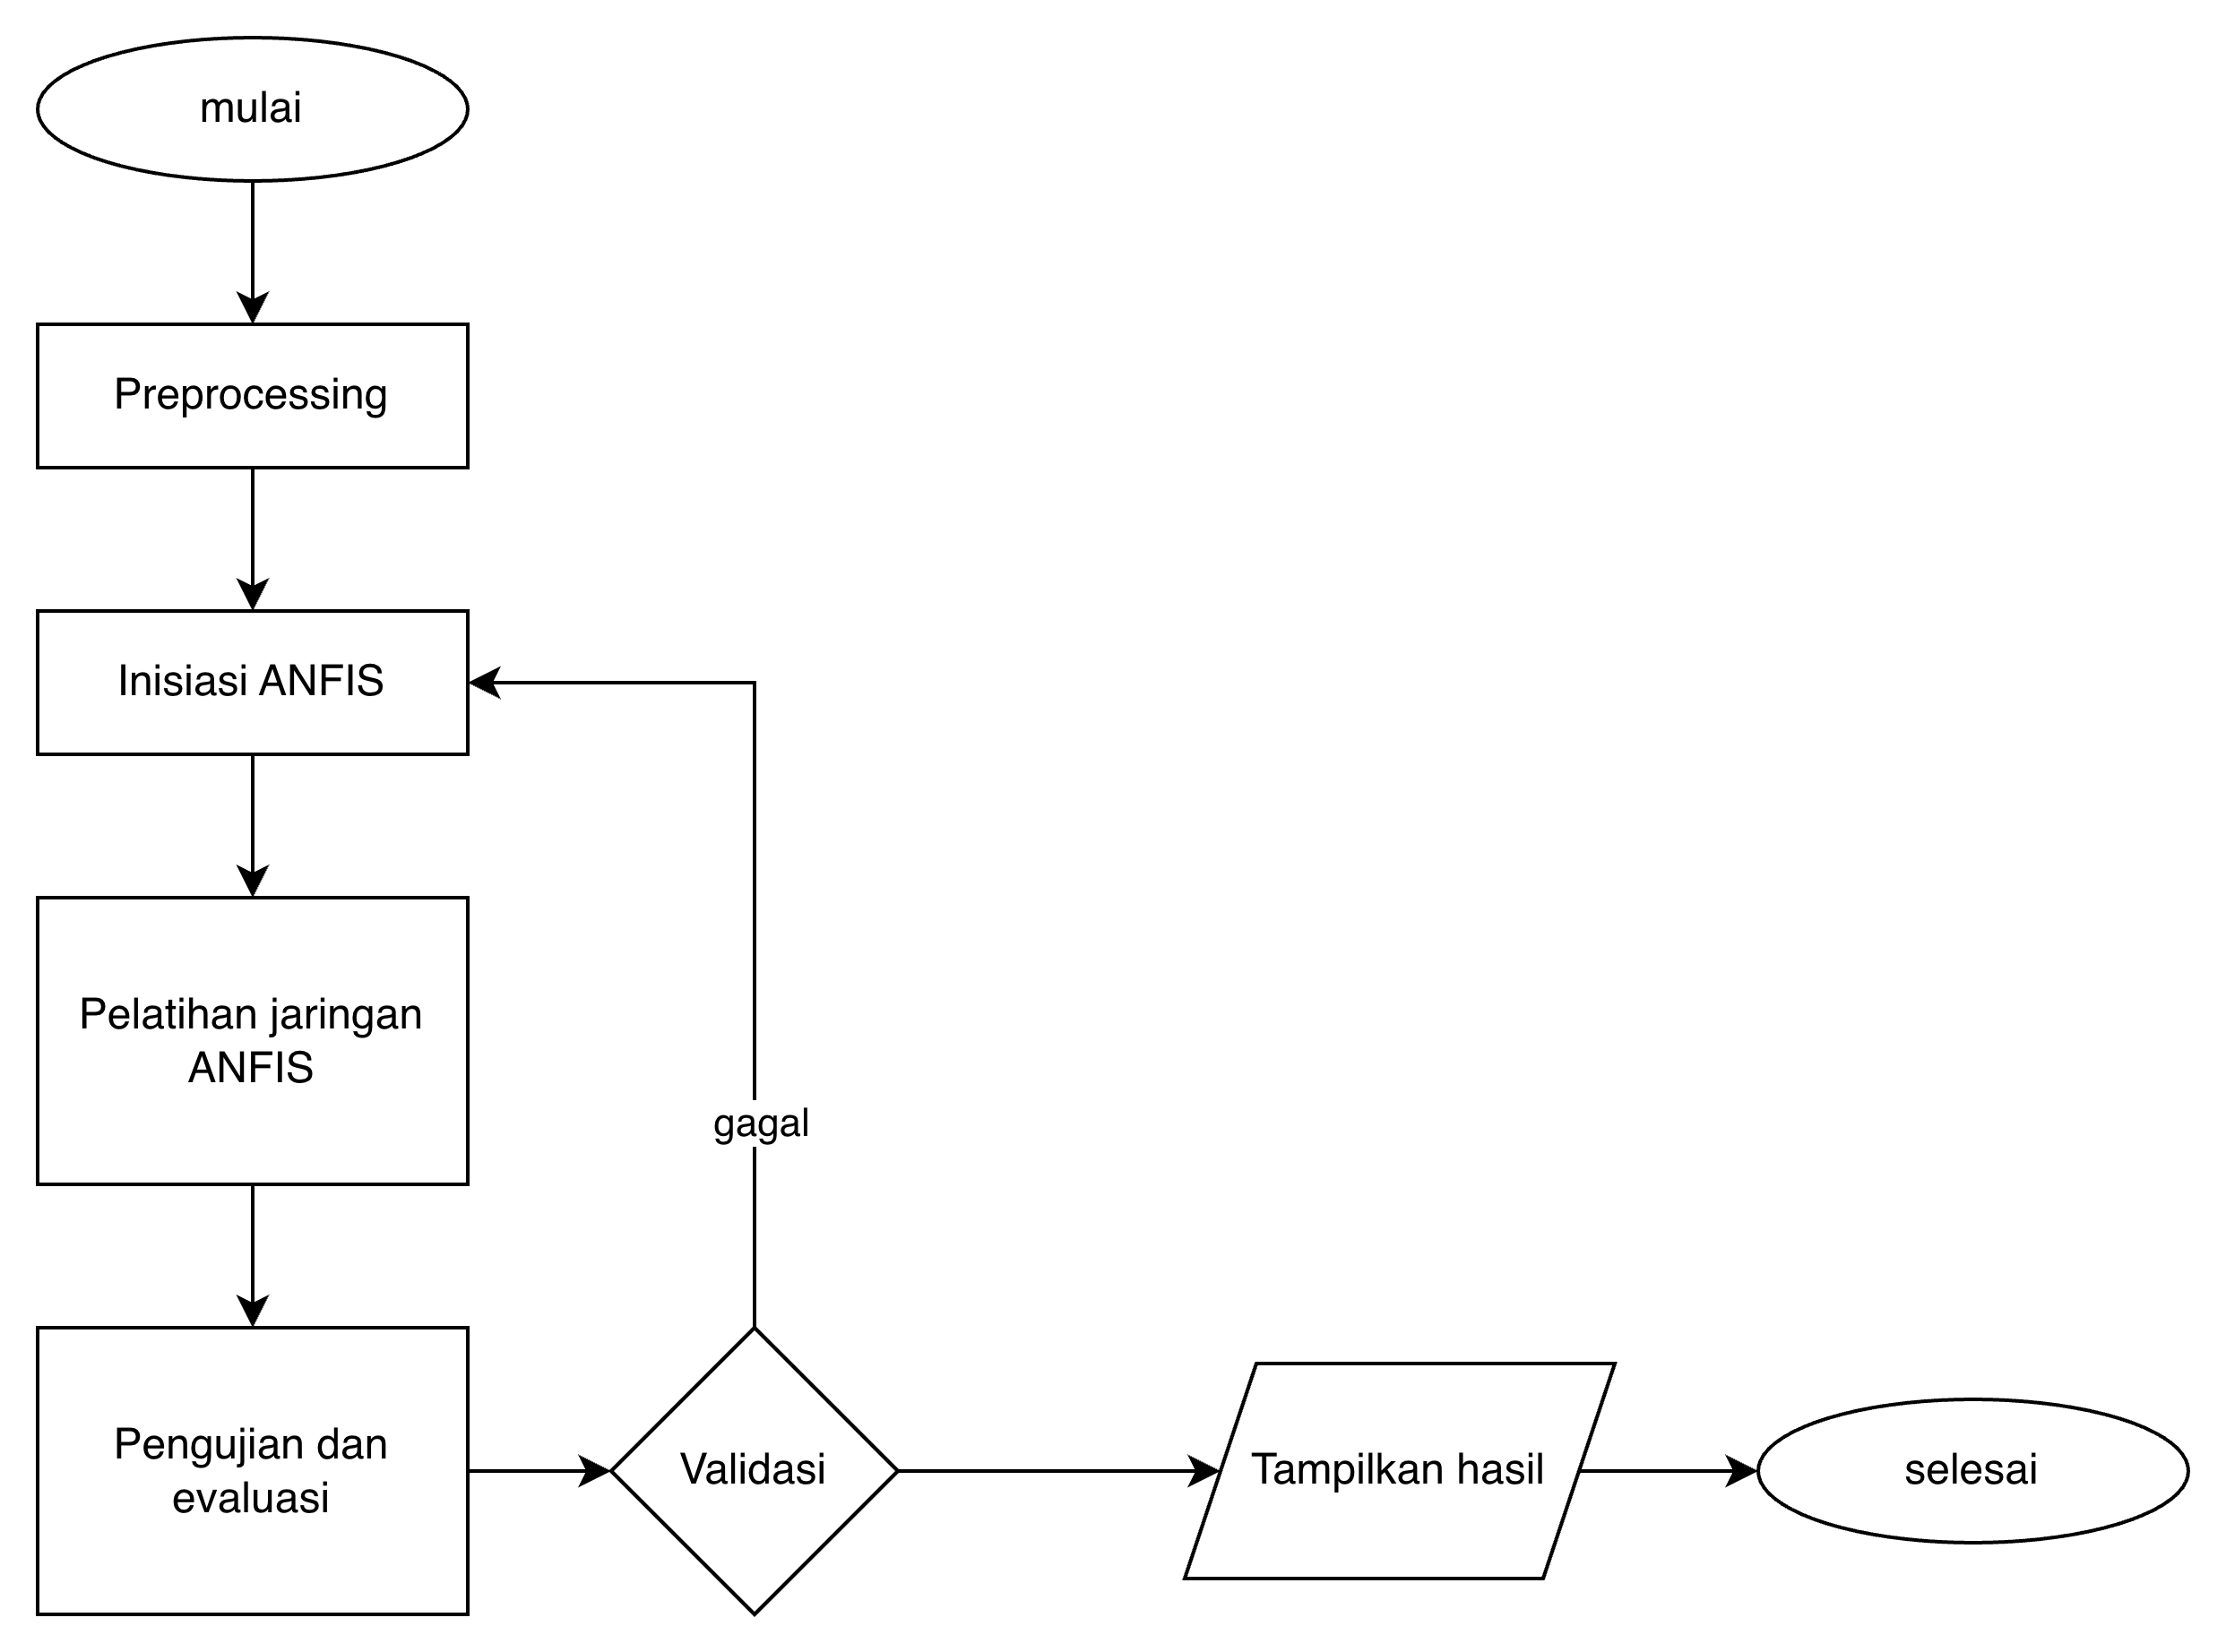
\includegraphics[width=0.8\textwidth]{flowchart.png}
    \caption{Flowchart}\label{fig:flowchart}
\end{figure}

Proses pelaksanaan komputasi sistem dibagi menjadi beberapa tahapan utama:
\begin{enumerate}
    \item \textbf{Tahap Input \& Preprocessing:} Memuat 1.030 sampel \textit{Concrete Compressive Strength Dataset}. Melakukan pembersihan data (\textit{h\-and\-ling missing values/outliers}) dan pembagian data (\textit{data splitting}) menjadi Data Training (80\%) dan Data Testing (20\%).
    \item \textbf{Tahap Inisialisasi FIS:} Inisiasi awal \textit{Fuzzy Inference S\-ys\-tem} (FIS) berdasarkan aturan \textit{grid partition} yang telah ditentukan pada perancangan basis arturan pada sesi~\ref*{rule_base}.
    \item \textbf{Tahap Pelatihan Hibrida (Hybrid Learning):} Proses optimasi parameter ANFIS dijalankan secara \textit{forward-backward pass}. Algoritma \textit{Least Squares Estimator} mengekstrak parameter konsekuen (Layer 4), sementara \textit{Backpropagation Gradient Descent} memperbaiki parameter premis fungsi keanggotaan (Layer 1).
    \item \textbf{Tahap Pengujian \& Evaluasi:} Model yang telah terlatih diuji menggunakan Data Testing (20\%) untuk memprediksi kuat tekan beton yang belum pernah dilihat oleh sistem.
    \item \textbf{Tahap Validasi Indeks Kinerja:} Performa akurasi diukur menggunakan metrik \textit{Root Mean Squared Error} (RMSE) dan Koefisien Determinasi ($R^2$). Jika nilai RMSE belum memenuhi ambang batas target, sistem akan kembali ke tahapan penyetelan ulang arsitektur \textit{membership function}.
\end{enumerate}